\chapter{Mathematical Foundation}

\section{Basics of Compressed Sensing}
As it was shortly mentioned in chapter~\ref{chapter:introduction}, a mathematical framework called compressed sensing (CS) revolutionized MR image acquisition process allowing reconstruction from much fewer k-space values \textit{under certain conditions} as it would be necessary according to the Nyquist criterion.

To realize this promise, first and foremost, the signal to be recovered must be sparse in some transform domain. Fortunately, natural images are intrinsically sparse in the Fourier domain and in many other wavelet domains, MR images are being no exception to that, and as MRI scanners operates on Fourier transform, the sparsity condition is always satisfied by the very nature of the imaging process. The other conditions, however, are less intuitive, hence in this section we attempt to give a quick overview of the most important definitions and theorems needed for basic understanding, based on the book~\cite{foucart_mathematical_2013}, and on the lectures of the course titled \textit{Compressive Sampling} at Technical University of Munich by Alihan Kaplan.

\subsection{Elementary Definitions}

Although the reader might be to be familiar with the most of these definitions, for the sake of completeness and clarity of notation used in this work, we present here a list of definitions of elementary constructs, restricting ourselves to mere formulations with short remarks omitting further explanation.

\begin{tight_equations}

\begin{definition}[norm]
A non-negative function $\norm{\cdot}: X \rightarrow [0, \infty)$ is called a norm, if 
\begin{enumerate}[label=\alph*)]
    \item $\norm{\mathbf{x}} = 0$ if and only if $\mathbf{x} = \mathbf{0}$,
    \item $\norm{\lambda \mathbf{x}} = \Vert \lambda \Vert \norm{\mathbf{x}}$ for all scalars $\lambda$ and all vectors $\mathbf{x} \in X$, and
    \item $\norm{\mathbf{x} + \mathbf{y}} \le \norm{\mathbf{x}} + \norm{\mathbf{y}}$ for all vectors $\mathbf{x, y} \in X$.
\end{enumerate}
\end{definition}

\begin{remark}
$X$ denotes a vector space on which the norm is defined. In MRI setting, however, $\mathbb{C}^N$ is the default vector space for computations, and therefore, we also define the following constructs in this space.
\end{remark}

\begin{definition}[$\ell_p$-norms for vectors]
The $\ell_p$-norm on $\mathbb{C}^N$ is defined for $1 \le p < \infty$ as
\begin{equation}\label{eq:p-norm}
\norm{\mathbf{x}}_p = \left(\sum_{j=1}^n |x_j|^p\right)^{\frac{1}{p}},
\end{equation}
and for $p = \infty$ as
\[\norm{\mathbf{x}}_\infty = \max_{j \in [n]} | x_j |.\]
For $0 < p < 1$, (\ref{eq:p-norm}) defines a quasinorm, which means that from the definition of the norm a) and b) holds, but c) is replaced by the weaker quasitriangle inequality
\[\norm{\mathbf{x} + \mathbf{y}}_p \le C\left(\norm{\mathbf{x}}_p + \norm{\mathbf{y}}_p\right)\]
with $C = 2^{\frac{1}{2}-1}$.
\end{definition}

\begin{remark}
Figure~\ref{fig:balls} is showing 2-dimensional balls defined by $\ell_p$-norm with various $p$ values.
\end{remark}

\begin{figure}
    \centering
    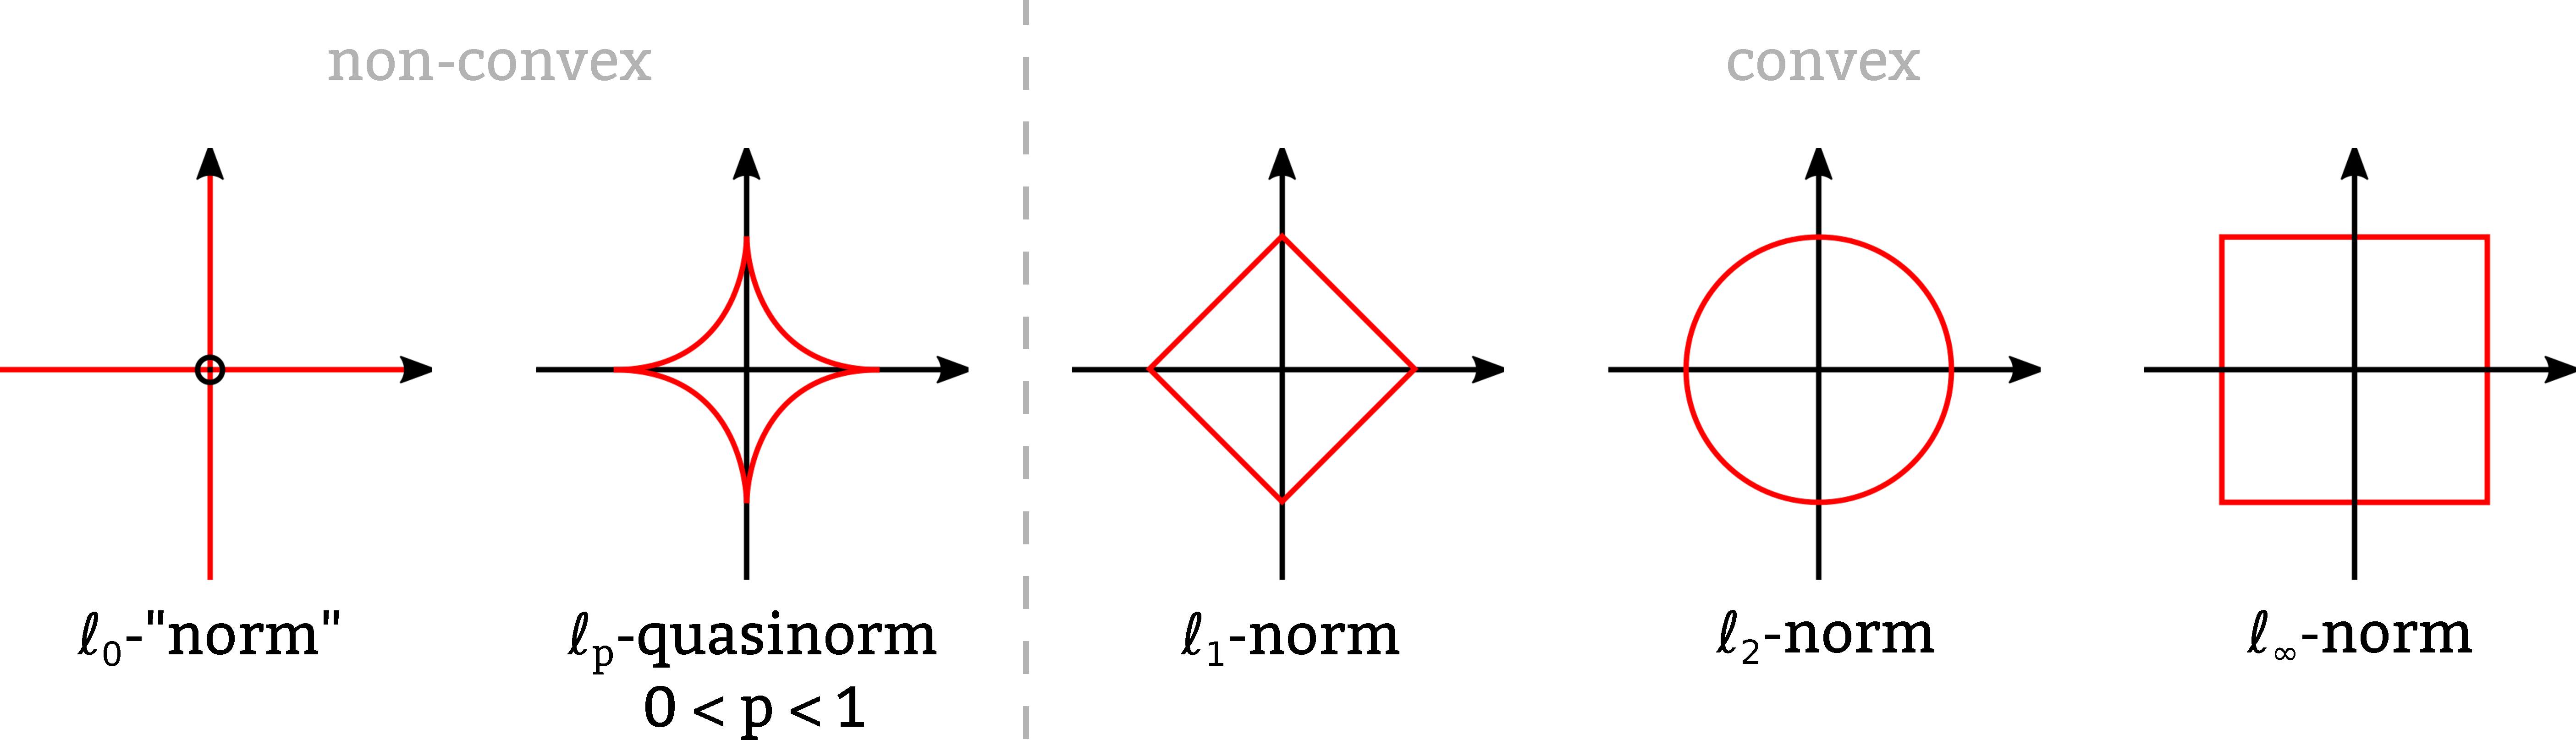
\includegraphics[width=\textwidth]{images/balls.pdf}
    \caption{\textbf{$\ell_p$ balls in 2D.}}
    \label{fig:balls}
\end{figure}

\begin{notation}
$[n]$ denotes the set of integers form $0$ to $n-1$.
\end{notation}

\begin{remark}
Using the schema above, it is impossible to have a proper norm for $p = 0$; nonetheless, is very common to define $\ell_0$-norm as the number of non-zero coordinates:
\[\norm{\mathbf{x}}_0 = \left| \left\{x_i \ne 0 : i \in [n]\right\}\right| \text{ where } \mathbf{x} \in \mathbb{C}^N.\]
Following this convention, $\norm{\cdot}_0$ always refers to that definition in the definitions and theorems below.
\end{remark}

\begin{definition}[sparsity]
We call a vector $s$-sparse, if at most $s$ of its entries are non-zero; i.e. $\norm{\mathbf{x}}_0 \le s$.
\end{definition}

\begin{notation}
By $\Sigma_s^N$ we denote the set of all s-sparse vectors in $\mathbb{C}^N$; that is,
\[\Sigma_s^N = \left\{\mathbf{x} \in \mathbb{C}^N : \norm{\mathbf{x}}_0 \le s \right\}.\]
\end{notation}

%\begin{notation}
%The solution set $\left\{\mathbf{x} \in \mathbb{C}^N : \mathbf{Ax} = \mathbf{y}\right\}$ is denoted by $L_\mathbf{A}(\mathbf{y})$ for a given $\mathbf{A} \in \mathbb{C}^{m \times N}$.
%\end{notation}

%\begin{definition}[unique sparse solution]
%A vector $\mathbf{x}_* \in \mathbb{C}^N$ is the unique $s$-sparse solution of equation $\mathbf{Ax} = \mathbf{y}$ with $\mathbf{A} \in \mathbb{C}^{m \times N}$ and $\mathbf{y} \in \mathbb{C}^m$, if $L_\mathbf{A}(\mathbf{y}) \cap \Sigma_s^N = \{\mathbf{x}_*\}$, in other words, it is the only $s$-sparse vector satisfying the  linear system defined by $\mathbf{A}$ and $\mathbf{y}$.
%\end{definition}

\begin{definition}[kernel/null space]
The kernel/null space of a matrix $\mathbf{A} \in \mathbb{C}^{m \times N}$ is defined as
\[ker(\mathbf{A}) = \left\{\mathbf{x} \in \mathbb{C}^N : \mathbf{Ax} = \mathbf{0}\right\}.\]
\end{definition}

\begin{theorem}[SVD]
For $\mathbf{A} \in \mathbb{C}^{m \times N}$, there exist unitary matrices $\mathbf{U} \in \mathbb{C}^{m \times m}$, $\mathbf{V} \in \mathbb{C}^{N \times N}$, and uniquely defined non-negative numbers $\sigma_1 \ge \sigma_2 \ge \ldots \ge \sigma_{min\{m,N\}} \ge 0$ called singular values of $\mathbf{A}$, such that 
\[\mathbf{A} = \mathbf{U \Sigma V^*} \text{ where } \mathbf{\Sigma} = diag[\sigma_1, \sigma_2, \ldots, \sigma_{min\{m,N\}}] \in \mathbb{R}^{m \times N}.\]
The process of obtaining these matrices is called Singular Value Decomposition (SVD).
\end{theorem}

\end{tight_equations}

\subsection{Formulation of the Problem}
In engineering settings, especially in signal processing context, engineers and scientist usually try first to model physical systems by a linear model because that way they describe the problem by a set of linear expressions, and then they can express it as a matrix-vector multiplication $\mathbf{Ax} = \mathbf{y}$, where vector $\mathbf{x}$ is the input of the system, vector $\mathbf{y}$ is the output (measured data), and $\mathbf{A}$ characterizes the measurement (thus it is often referred to as \textit{measurement matrix}). A very common task then is to recover the input consisting of $N$ variables from the measurement data, and generally the number of measurements $m$ must obey $m > N$, otherwise the linear system is underdetermined, and hence there exist infinitely many solutions. In case of MRI setting, this statement corresponds to already mentioned Nyquist criterion that requires the sampling frequency in k-space to be twice as the highest frequency in the image space (vid. $k_{FOV} = 2 \cdot k_{max}$ in section~\ref{section:accelerated}).

And that is the point when compressed sensing comes into play claiming that given a \textit{proper} measurement matrix $\mathbf{A}$, the problem

\begin{equation}
    \tag{P\textsubscript{0}}\label{eq:P_0}
    \min_{\mathbf{z} \in \mathbb{C}^N} \norm{\mathbf{z}}_0 \text{ subject to } \mathbf{Az} = \mathbf{y} = \mathbf{Ax}
\end{equation}
have a unique $s$-sparse solution with $s \ll N$. This optimization problem is often referred to as (\ref{eq:P_0}). The number of necessary measurement, however, still a difficult question. There are theoretical results stating that $m = 2s$ is the lower bound for a perfect recovery~\citationneeded and that a stable recovery (later explained) occurs with high probability with $m \ge C s log(N / m)$ for random measurement matrices~\citationneeded, but in practice, reconstruction algorithms struggle to reach these theoretical limits (albeit, the achieved $m$ is still drastically improved compared to the Nyquist sampled case).

The main reason why the optimal bounds are usually not reached is that the measurement matrices of real life systems have often have less favorable properties as random matrices and, more importantly, (\ref{eq:P_0}) is a NP-hard problem~\citationneeded; thus, only relaxations can be solved. The most commonly used relaxations are the so called $\ell_1$ minimization or Basis Pursuit (BP)~\citationneeded defined as
\begin{equation}
    \tag{P\textsubscript{1}}\label{eq:P_1}
    \min_{\mathbf{z} \in \mathbb{C}^N} \norm{\mathbf{z}}_1 \text{ subject to } \mathbf{Az} = \mathbf{y},
\end{equation}
the Basis Pursuit DeNoising (BPDN)~\citationneeded formulated as

\begin{equation}
    \tag{P\textsubscript{1}, \texteta}\label{eq:P_1_noisy}
    \min_{\mathbf{z} \in \mathbb{C}^N} \norm{\mathbf{z}}_1 \text{ subject to } \norm{\mathbf{Az} - \mathbf{y}}_2 \le \eta,
\end{equation}
and the LASSO (Least Absolute Shrinkage and Selection Operator)~\citationneeded problem expressed by
\[\min_{\mathbf{z} \in \mathbb{C}^N} \norm{\mathbf{Az} - \mathbf{y}}_2 \text{ subject to } \norm{\mathbf{z}}_1 \le s.\]
By the aid of a Lagrangian multiplier $\lambda$, the latter two can be transformed to the same unconstrained minimization problem
\[\min_{\mathbf{z} \in \mathbb{C}^N} \norm{\mathbf{Az} - \mathbf{y}}_2 + \lambda \norm{\mathbf{z}}_1.\]

\subsection{Conditions and Guarantees}
While $\ell_1$-relaxation (often referred to as (\ref{eq:P_1}) problem) might be appealing as it can be solved efficiently in polynomial time, it needs a more careful approach to guarantee that the minimum of the $\ell_1$ problem is also a solution of (\ref{eq:P_0}). The $\ell_2$-relaxation, for example, always has a unique solution, but this solution is not necessarily sparse (for a figurative illustration, see fig.~\ref{fig:sparse_solution} and fig.~\ref{fig:3D_l1_min}). In contrast, $\ell_1$ problem has a solution which is both unique and $s$-sparse given that the matrix $\mathbf{A}$ fulfills the so called \textit{null space property} of order $s$, introduced by Cohen, Dahmen and DeVore in~\cite{cohen_compressed_2009}.

\begin{figure}[tb]
    \centering
    \begin{minipage}{.63\textwidth}
        \centering
        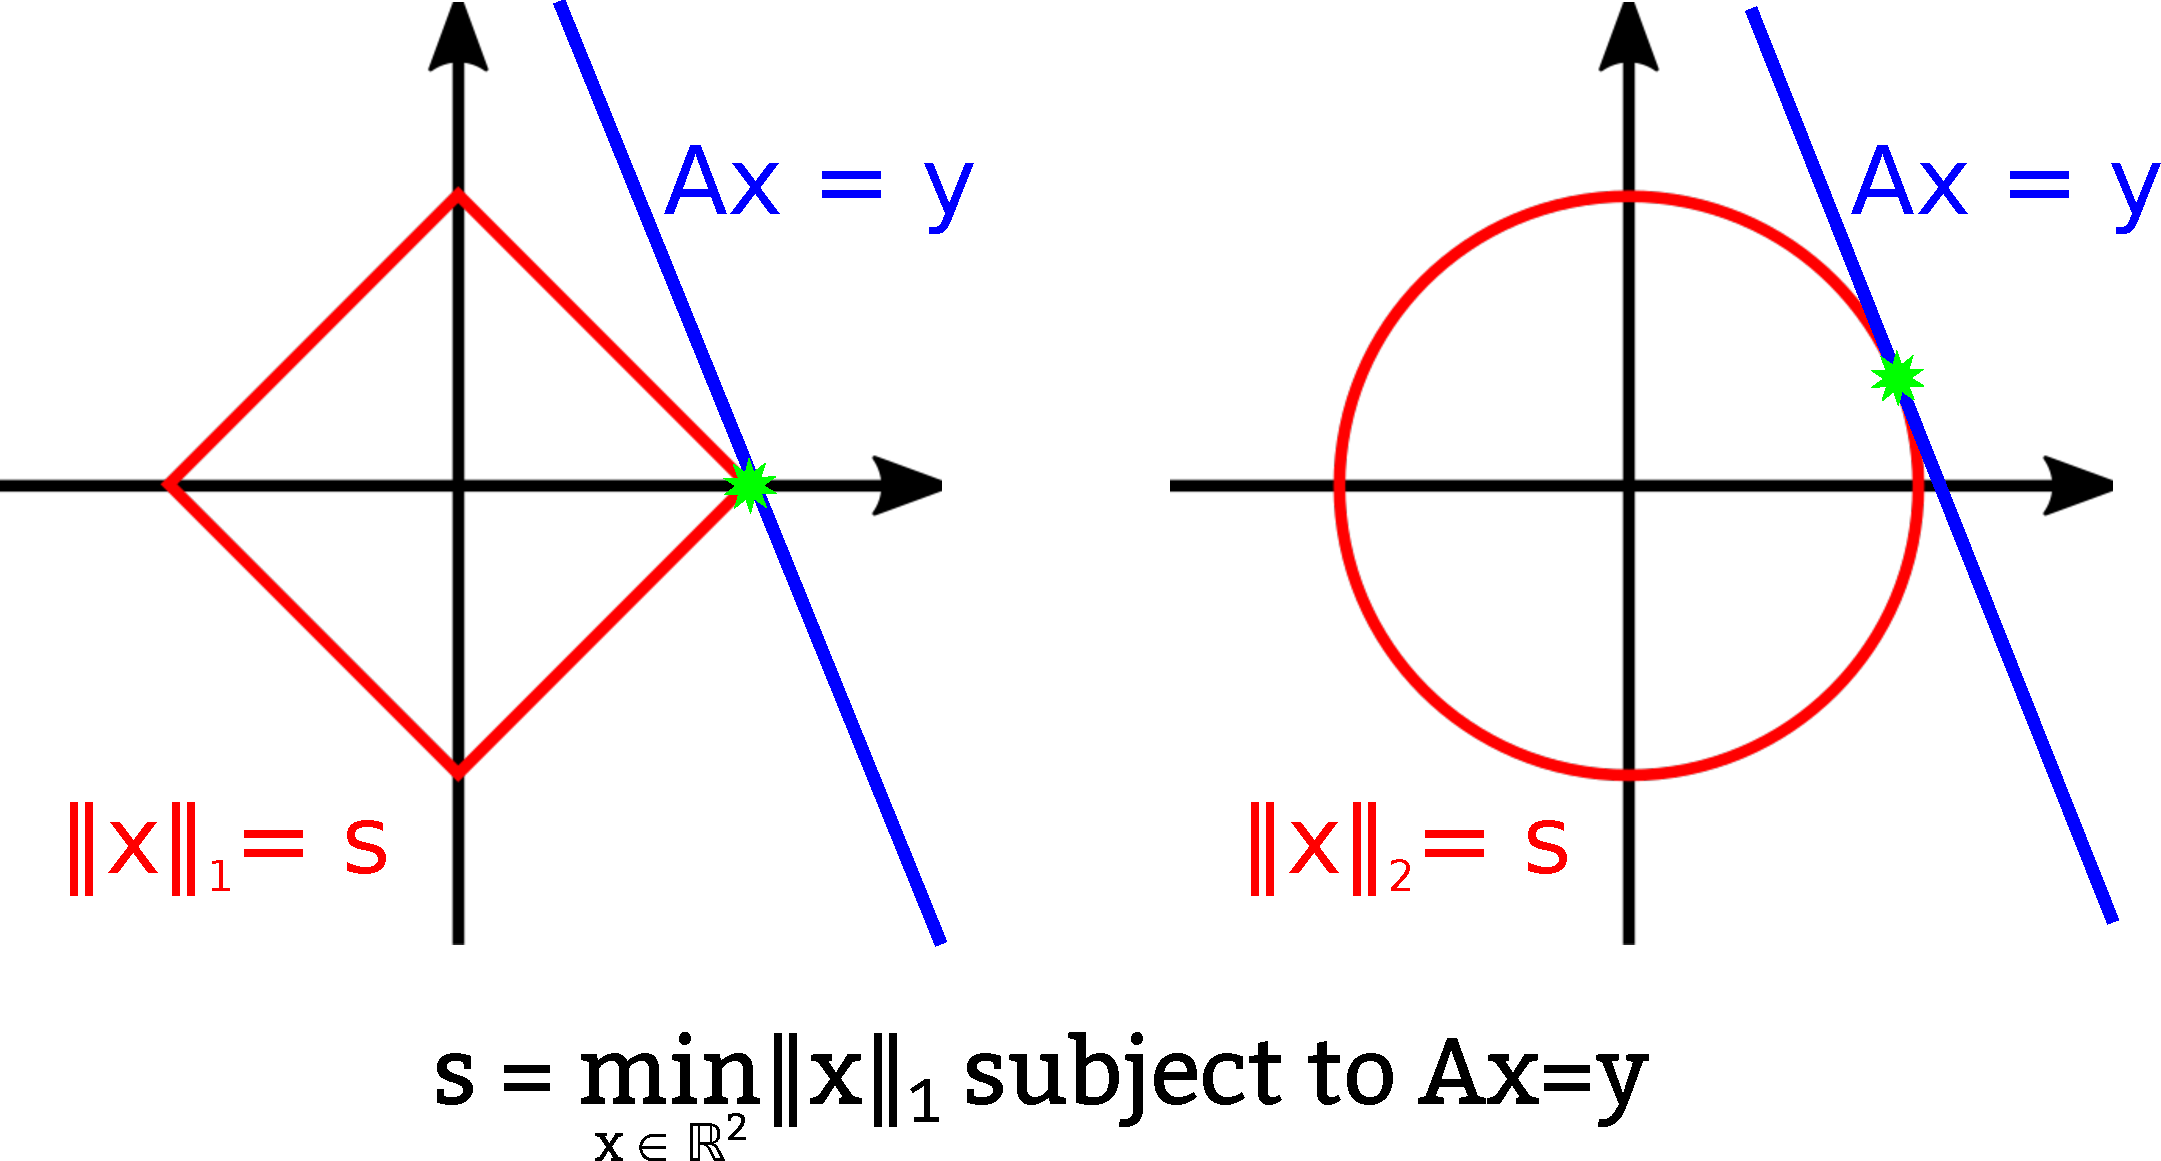
\includegraphics[width=0.7\linewidth]{images/sparse_solution.pdf}
        \caption{\textbf{Solution of $\ell_1$ and $\ell_2$ minimization problems.} Matrix $\mathbf{A} \in \mathbb{R}^{1 \times 2}$ is an underdetermined linear system, and the task is to find $\mathbf{x} \in \mathbb{R}^2$ with minimal $\ell_1$-norm such that it satisfies the equation $\mathbf{Ax} = \mathbf{y}$ for fixed $\mathbf{y} \in \mathbb{R}$. The number of solutions are infinite (all points along the blue line), and the unique solution of minimization problem is marked with a green star. Note that $\ell_1$ minimization gives sparse solution, while $\ell_2$ minimization is not sparsity seeking.}
        \label{fig:sparse_solution}
    \end{minipage}%
    \hspace{0.02\textwidth}
    \begin{minipage}{0.34\textwidth}
        \centering
        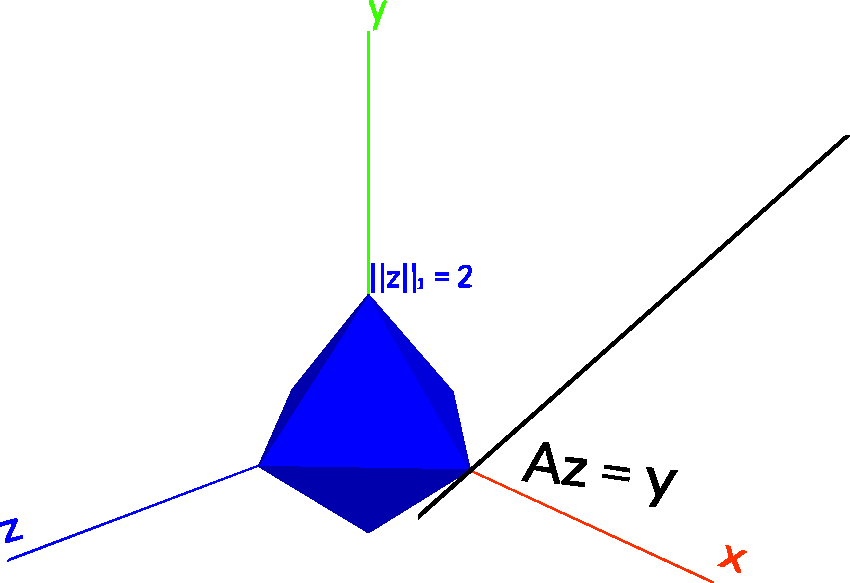
\includegraphics[width=\linewidth]{images/3D_l1_min.pdf}
        \caption{\textbf{$\ell_1$ minimization in 3D.} This figure demonstrates the sparsity seeking nature of $\ell_1$ minimization in a 3-dimensional space. The image is taken from the interactive demo available at \url{https://hakkelt.github.io/CS-demo/}}
        \label{fig:3D_l1_min}
    \end{minipage}
\end{figure}

\begin{definition}[NSP]
A matrix $\mathbf{A} \in \mathbb{C}^{m \times N}$ is said to satisfy the null space property (NSP) of order $s$, if for any set $S \subset [N]$ with $|S| = s$
\[\norm{\mathbf{v}_S}_1 < \norm{\mathbf{v}_{S^C}}_1 : \forall \mathbf{v} \in ker(\mathbf{A})  \setminus \{\mathbf{0}\}.\]
\end{definition}

\begin{notation}
For a vector $\mathbf{v} \in \mathbb{C}^N$ and a set $S \subset [N]$, we denote by $\mathbf{v}_S$ either the vector in $\mathbb{C}^{|S|}$ which is the restriction of $\mathbf{v}$ to the indices in $S$, or the vector in $\mathbb{C}^N$ which coincides with $\mathbf{v}$ on the indices in $S$ and is zero elsewhere. Similarly, $\mathbf{v}_{S^C}$ means the same with the complement of $S$.
\end{notation}

\begin{theorem}
Given a matrix $\mathbf{A} \in \mathbb{C}^{m \times N}$, every $s$-sparse vector $\mathbf{x} \in \Sigma_s^N \subset \mathbb{C}^N$ is the unique solution of (\ref{eq:P_1}) with $\mathbf{y} = \mathbf{Ax}$ if and only if $\mathbf{A}$ satisfies the NSP of order $s$.
\end{theorem}

\begin{remark}
This theorem shows that for every $\mathbf{y} = \mathbf{Ax}$ with $s$-sparse $\mathbf{x}$, the $\ell_1$-minimization (\ref{eq:P_1}) actually solves the $\ell_0$-minimization (\ref{eq:P_0}) when the NSP of order $s$ holds.
\end{remark}

Although NSP is a formidable construct that allows relatively easy and straightforward proofs, in realistic settings, signals are rarely sparse, but rather \textit{almost} $s$-sparse vectors, meaning that the most part of the energy of the signal is concentrated in $s$ coefficients with the the largest values. To involve these cases in the compressed sensing framework, an extension of NSP is used, called \textit{stable NSP}. Proving the stable NSP property, one can then approximate the almost $s$-sparse signal with the \textit{best $s$-term approximation} having a tight bound on the error term.

\begin{definition}[$\ell_p$-error of best $s$-term approximation]
For $p > 0$, the $\ell_p$-error of best $s$-term approximation to a vector $\mathbf{x} \in \mathbb{C}^N$ is defined by
\[\sigma_s(\mathbf{x})_p = \inf\left\{\norm{\mathbf{x} - \mathbf{z}}_p : \mathbf{z} \in \Sigma_s^N\right\}.\]
\end{definition}

\begin{remark}
The  infimum is always achieved by an $\mathbf{z} \in \Sigma_s^N$ whose non-zero entries equal the $s$ largest absolute entries of $\mathbf{x}$.
\end{remark}

\begin{definition}[stable NSP]
A matrix $\mathbf{A} \in \mathbb{C}^{m \times N}$ is said to satisfy the stable NSP with constant $0 < \rho < 1$ of order $s$, if for any set $S \subset [N]$ with $|S| = s$
\[\norm{\mathbf{v}_S}_1 \le \rho \norm{\mathbf{v}_{S^C}}_1 : \forall \mathbf{v} \in ker(\mathbf{A}).\]
\end{definition}

\begin{theorem}
The matrix $\mathbf{A} \in \mathbb{C}^{m \times N}$ satisfies the stable NSP with constant $0 < \rho < 1$ of order $s$ if and only if for any set $S \subset [N]$ with $|S| = s$
\begin{equation}\label{eq:stable_nsp}
    \norm{\mathbf{z} - \mathbf{x}}_1 \le \frac{1 + \rho}{1 - \rho} \left(\norm{\mathbf{z}}_1 - \norm{\mathbf{x}}_1 + 2\norm{\mathbf{x}_{S^C}}\right)
\end{equation}
holds for any set $S \subset [N]$ with $|S| = s$ and for all vectors $\mathbf{x,z} \in \mathbb{C}^N$ with $\mathbf{Az} = \mathbf{Ax}$.
\end{theorem}

\begin{remark}
The estimation (\ref{eq:stable_nsp}) can be upper-bounded by means of the $\ell_1$-error of best $s$-term approximation $\sigma_s(\mathbf{x})_1$ as
\[\norm{\mathbf{z} - \mathbf{x}}_1 \le \frac{1 + \rho}{1 - \rho} \left(\norm{\mathbf{z}}_1 - \norm{\mathbf{x}}_1 + 2\norm{\mathbf{x}_{S^C}}\right) \le 2 \cdot \frac{1 + \rho}{1 - \rho}\sigma_s(\mathbf{x})_1.\]
\end{remark}

The significance of this theorem is that it implies that having the stable NSP fulfilled, the unique $s$-sparse solution $\mathbf{z}$ of (\ref{eq:P_1}) with $\mathbf{y} = \mathbf{Ax}$ approximates the vector $\mathbf{x}$ with a bounded $\ell_1$-error. Therefore, by a good approximation of the sparsity $s$ of the signal and an upper bound $\epsilon$ of $\sigma_s(\mathbf{x})_1$ (both can be inferred by the statistics of the signal), one can construct or select a measurement matrix $\mathbf{A}$ such that the solution of \textit{any} algorithm solving (\ref{eq:P_1}) is an approximation of the input signal with the maximal error of
\[\frac{1 + \rho}{1 - \rho} \cdot 2\epsilon,\]
where $\rho$ depends only on the measurement matrix and $\epsilon$ is a small number because only little energy is stored in the entries contributing the the $\ell_p$-error of best $s$-term approximation.
Practically that means that by the careful design of the measurement, arbitrary precision recovery is possible (having Nyquist sampling as a special case for guaranteed perfect recovery), and that in case of almost $s$-sparse signals, the number of measurements can be drastically reduced without significant amount of error introduced.

Finally, this construct can be further extended  to handle noisy measurement: proving the \textit{robust NSP} for the measurement matrix, the same guaranties apply to the $\ell_1$-error as in case of stable recovery, extended by an extra term characterizing the noise on the measurement. As a result, arbitrary precision is allowed for arbitrary optimization algorithm capable of solving (\ref{eq:P_1_noisy}) given a measurement matrix satisfying the \textit{robust NSP}.

\begin{definition}[robust NSP]
A matrix $\mathbf{A} \in \mathbb{C}^{m \times N}$ is said to satisfy the robust NSP with constants $0 < \rho < 1$ and $0 < \tau$ of order $s$, if for any set $S \subset [N]$ with $|S| = s$
\[\norm{\mathbf{v}_S}_1 \le \rho \norm{\mathbf{v}_{S^C}}_1 + \tau \norm{\mathbf{Av}}_2 : \forall \mathbf{v} \in \mathbb{C}^N.\]
\end{definition}

\begin{remark}
Note that $\mathbf{v}$ is not required to be in $ker(\mathbf{A})$.  In fact, if $\mathbf{v} \in ker(\mathbf{A})$, then $\mathbf{Av} = \mathbf{0}$, and we obtain the definition of stable NSP. Therefore, the robust NSP implies stable NSP.
\end{remark}

\begin{theorem}
The matrix $\mathbf{A} \in \mathbb{C}^{m \times N}$ satisfies the robust NSP with constants $0 < \rho < 1$ and $0 < \tau$ of order $s$ if and only if
\begin{equation}\label{eq:robust_nsp}
    \norm{\mathbf{z} - \mathbf{x}}_1 \le \frac{1 + \rho}{1 - \rho} \left(\norm{\mathbf{z}}_1 - \norm{\mathbf{x}}_1 + 2\norm{\mathbf{x}_{S^C}}\right) + \frac{2\tau}{1-\rho}\norm{\mathbf{A(z-x)}}_2
\end{equation}
holds for any set $S \subset [N]$ with $|S| = s$ and for all vectors $\mathbf{x,z} \in \mathbb{C}^N$ with $\mathbf{Az} = \mathbf{Ax}$.
\end{theorem}

\begin{remark}
Supposing that a matrix $\mathbf{A} \in \mathbb{C}^{m \times N}$ satisfies the robust NSP of order $s$, (\ref{eq:robust_nsp}) implies that for any $\mathbf{x} \in \mathbb{C}^N$, a solution $\mathbf{z}$ of (\ref{eq:P_1_noisy}) with $\norm{\mathbf{Ax - y}} \le \eta$ approximates $\mathbf{x}$ with $\ell_1$-error \footnote{Number $4$ in the numerator of the error term at (\ref{eq:error_bound}) is not a typo as one would expect, but a counterintuitive result of some basic arithmetics leading to this expression.}
\begin{equation}\label{eq:error_bound}
    \norm{\mathbf{z} - \mathbf{x}}_1 \le 2 \cdot \frac{1 + \rho}{1 - \rho}\sigma_s(\mathbf{x})_1 + \frac{4\tau}{1-\rho}\eta.
\end{equation}
\end{remark}

\begin{remark}
The main problem with the NSP is that proving it is actually NP-hard in general. Hence, the \textit{restricted isometry property (RIP)} is more commonly used in theoretical works because it is easier to handle, and at the same time it implies stable NSP.
\end{remark}

\subsection{The Connection Between CS and MRI}
Although it is not always trivial to apply the compressed sensing scheme to different measurement methods, MRI is in a lucky position with the Fourier transform in its core as random partial discrete Fourier transform (i.e., selecting $m$ rows randomly with uniform distribution from the $N$ rows, or in other words, observing only $m$ entries of the Fourier transform) is proved to satisfy the RIP and thus also the NSP~\cite{fornasier_theoretical_2010}. That discovery has enormous significance as is offers a way to speed up the inherently slow MRI measurements by measuring only a few randomly selected points from the k-space, and then solve the $\ell_1$-minimization problem via an arbitrarily selected optimization algorithm.

\begin{figure}[tb]
    \centering
    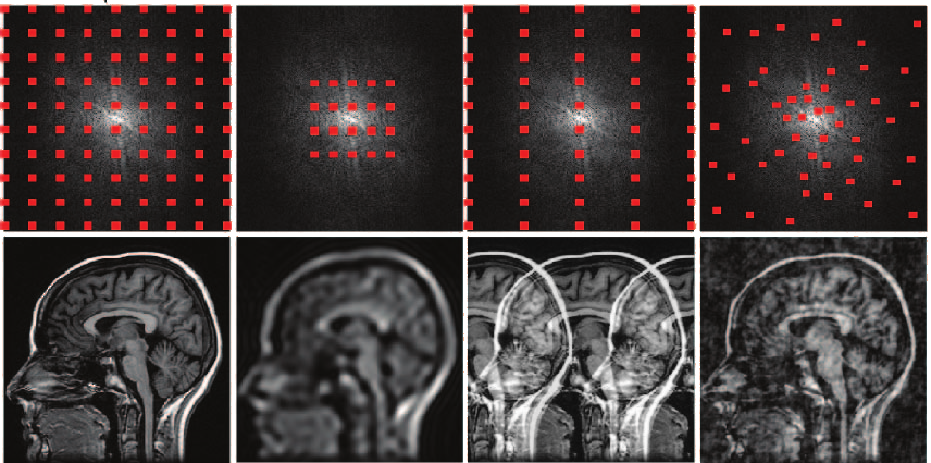
\includegraphics[width=\linewidth]{images/random_sampling2.png}
    \caption{\textbf{Connection between the sampling pattern and the introduced inference.} Using inverse DFT replacing the missing values with zeros leads to different type of undersampling artifacts. Sampling only the center reduces the resolution, undersampled equispaced scheme adds shifted copies of the signal to the recovered image, and random sampling spreads the inference uniformly. Source: Adapted from~\cite{lustig_compressed_2008}.}
    \label{fig:random_sampling_images}
\end{figure}

One can think of this recovery scheme as a denoising or inference cancelling process where the noise/inference to be removed is the sum of undersampling artifacts predicted by Nyquist-Shannon theorem. If we use an equispaced sampling pattern, then the resulted noise is basically shifted copies of the signal and hence recovery of the original signal is impossible as each replica is an equally likely candidate. In contrast, random sampling "spreads" the noise uniformly over the image, so the inference acts mostly like white noise (see fig.~\ref{fig:random_sampling_images}). This approach is particularly appealing as countless denoising algorithms exists, and as many of them are based on minimization of the $\ell_1$-norm of the transform of signal, these methods provide a convenient way to solve (\ref{eq:P_1}) problem. The transform used is always depends on the type of image in interest: MR angiograms (imaging technique visualizing blood vessels) are sparse even in the image domain, but edge detection algorithms like finite differences transform (that leads to the well-known total variation (TV) penalty) can further enhance sparsity (fig.~\ref{fig:MRA}); brain images have a sparse representation in various wavelet transformations~\ref{fig:brain_wavelet}, and dynamic MR images tend to be sparse after temporal Fourier transform is applied.

\begin{figure}
    \centering
    \begin{minipage}[t]{0.65\linewidth}
        \centering
        \begin{tabular}{c}
            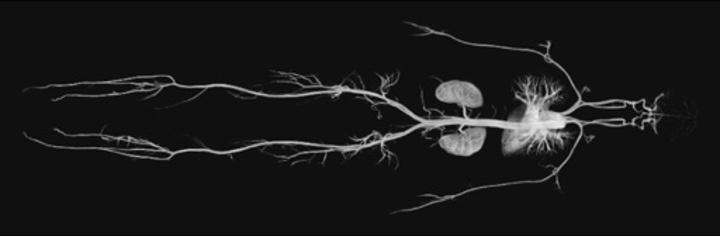
\includegraphics[width=0.95\linewidth]{images/MRI-Angiography.jpg}
            \\
            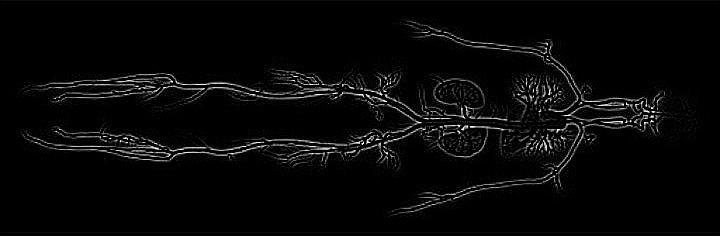
\includegraphics[width=0.95\linewidth]{images/MRI-Angiography_edges.jpg}
        \end{tabular}
        \caption{\textbf{MR angiograms} (MR images tuned to show blood vessels) are intrinsically sparse even in image domain (top image), but sparseness can be further improved by edge detection algorithms (botton image) because only the morphology of the blood vessels are diagnostically relevant. Source: Adapted from~\cite{noauthor_mri_nodate}.}
        \label{fig:MRA}
    \end{minipage}
    \hspace{0.02\linewidth}
    \begin{minipage}[t]{0.31\linewidth}
        \centering
        \begin{tabular}{c}
            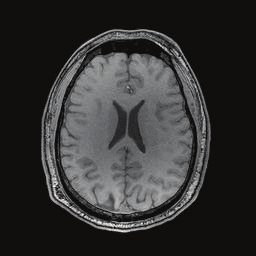
\includegraphics[width=0.65\linewidth]{images/brain_MRI.png}
            \\ 
            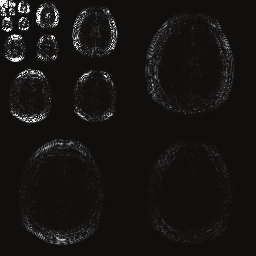
\includegraphics[width=0.65\linewidth]{images/brain_MRI_wavelet.png}
        \end{tabular}
        \caption{\textbf{MRI images of the brain} are not sparse in image domain, but they are in various wavelet transformations. Source:~\cite{zhao_compressed_2014}.}
        \label{fig:brain_wavelet}
    \end{minipage}
\end{figure}

A truly random sampling in the k-space, however, is generally impractical due to hardware and physiological constraints. For example, the sampling must follow smooth lines and curves and be robust to real-life situations such as motion artifacts. Also, a uniform random distribution of samples in the spatial-frequency domain does not take into account the energy distribution of MR images in k-space. Therefore it makes more sense to opt for a nonuniform variable density sampling matching energy distribution in k-space. Precisely, we should consider having more samples from the central part of the frequency domain and less high frequency components. Consequently, carefully designed pseudo-random sampling trajectories are utilized in practice. To quantify  evaluate the "randomness" of the trajectories, authors of~\cite{lustig_compressed_2008} and~\cite{lustig_sparse_2007} suggested using point spread function (PSF) to measure the desirable incoherence of the aliasing interference, defined as
\[PSF = (\mathbf{e}_j^* \mathcal{F}_u^* \mathcal{F}_u \mathbf{e}_i)_{i,j}\]
where $\mathcal{F}_u$ is the undersampling Fourier transform operator, $\mathbf{e}_i$ and $\mathbf{e}_j$ are of the natural basis having $0$ in each coordinate except the $i$-th and $j$-th position, resprectively, where $1$ is located. Thus, $PSF_{i,j}$ measures the contribution of a unit-intensity pixel at the $i$-th position of the image to the $j$-th position in the k-space. In case of fully sampled measurement, the $PSF$ is an identity matrix, and undersampling induces non-zero off-diagonal terms. Figuratively speaking, $PSF$ measures the leakage of energy from a Kronecker delta input. Figure~\ref{fig:trajectory_coherence} is showing $PSF$ for a central pixel for a couple sampling trajectories. This quantitiy then can serve as a simple measure for the overall incoherence by calculating the sidelobe-to-peak ratio:
\[SPR = \max_{i \ne j} \left|\frac{PSF_{i,j}}{PSF_{i,i}}\right|.\]
As a result, the design of an incoherent sampling trajetory aims to minimize $SPR$.

\begin{figure}
    \centering
    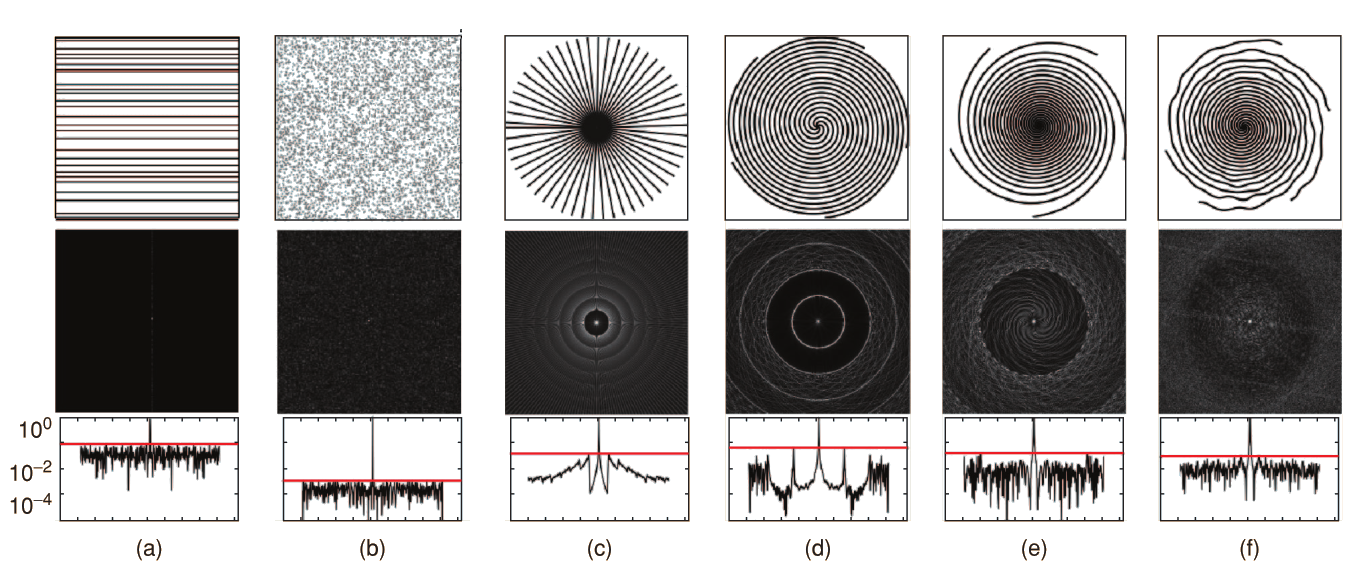
\includegraphics[width=\linewidth]{images/PSF_trajectories.png}
    \caption{$PSF$ of the central pixel for various sampling trajectories: (a) randomly chosen horizontal lines, (b) uniformly selected random points, (c) radial, (d) uniform spirals, (e) variable density spirals, and (f) variable density perturbed spirals. The red line marks the overall coherence level. Source: Adapted from~\cite{lustig_compressed_2008}.}
    \label{fig:trajectory_coherence}
\end{figure}

\section{Gradient Methods}

My slideshow about first order methods: \url{https://docs.google.com/presentation/d/1tIZSSfzzHUgo9tlKlmhSUCCWD3ynzyZwnWtpBUe--6g/edit}

\subsection{Gradient Descent}
From Cauchy to recent explosion of optimization algorithm.

The nonlinear conjugate gradient method is mainly based on the same idea as gradient descent (GD) method: That method can be imagined as a hiker trying to get down from a mountain and that hiker always follows the steepest direction; i.e., he or she is moving along the negative gradient in each time step. On the other hand, while the basic GD is easy to understand, fairly efficient, and widely used method to solve unconstrained optimization problems, it has also its drawbacks compared to other variants of the method. The three main problems are 1) the optimal step size, 2) curved "valleys", and 3) flat areas on the cost function surface. Fig.~\ref{fig:grad_desc_problem} shows an example where the inappropriate step size and a "curved valley" produce zigzagging motion, and slow convergence as a result, which is slowed even further when the flat area in the bottom of that valley is reached.

\begin{figure}
    \centering
    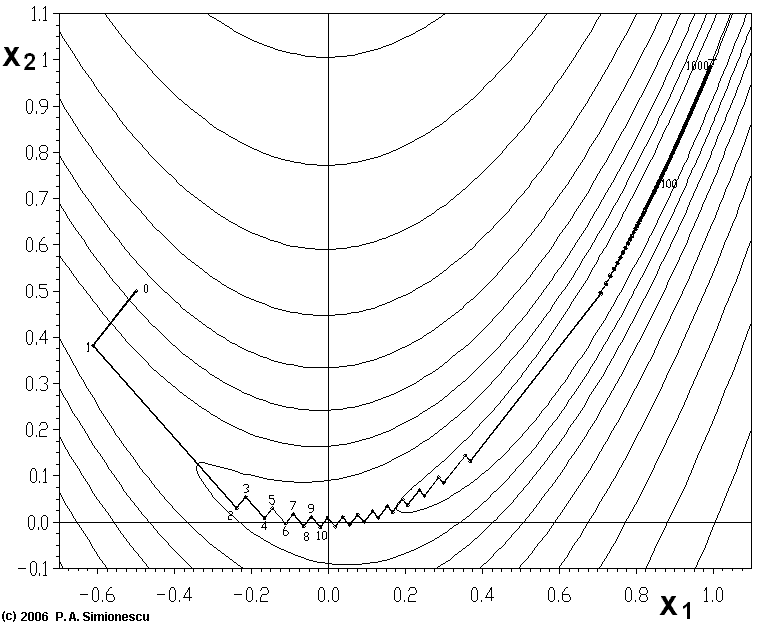
\includegraphics[width=0.3\linewidth]{images/project with Wiem/Banana-SteepDesc.png}
    \caption{Example of the effect of inappropriate step size, "curved valley" and flat area: slow convergence. Image from Wikipedia.org.}
    \label{fig:grad_desc_problem}
\end{figure}

Why would second order methods speed up convergence and why aren't we able to apply them to our problem.

\subsection{Conjugate Gradient}
How do they work, and when can conjugate gradient outperform gradient descent

\subsection{Conjugate Gradient Method}
To overcome the drawbacks of the basic GD method, one can use the conjugate gradient method (CG) that is an improved version of the basic GD method: in that case, the direction of movement must be conjugate to the previous directions. Two non-zero vectors $\mathbf{u}$ and $\mathbf{v}$ are conjugate (with respect to some $\mathbf{A}$ matrix), if $$\mathbf{u}^T\mathbf{Av} = \mathbf{0}.$$
Let us consider the following linear system as the subject of optimization:
$$\mathbf{Ax} = \mathbf{b},$$
where $\mathbf{A} $is symmetric, positive-definite and real matrix, and $\mathbf{b}$ is also known.

\subsubsection{As a direct method} Since $\mathbf{A}$ is symmetric and positive-definite, it defines an inner product:
$$\langle \mathbf{u}, \mathbf{v} \rangle_\mathbf{A} := \mathbf{u}^T\mathbf{Av}$$
Using that inner product, it is possible to find $n$ pairwise conjugate vectors: $\mathcal{P} = \{\mathbf{p}_1,...\mathbf{p}_n\}$. Then $\mathcal{P}$ forms a basis in $\mathbb{R}^n$, so the solution ($\mathbf{x_*}$) of optimization problem can be represented in terms of that basis:
\begin{equation} \label{eq:direct_method}
    \mathbf{x_*} = \sum_{i=1}^{n} \alpha_i \mathbf{p}_i.
\end{equation}
Left multiplying both sides with $\mathbf{p}_k^T \mathbf{A}$ we get:
$$\mathbf{p}_k^T\mathbf{Ax_*} = \sum_{i=1}^{n} \alpha_i \mathbf{p}_k^T \mathbf{A} \mathbf{p}_i = \sum_{i=1}^{n} \alpha_i \langle \mathbf{p}_k, \mathbf{p}_i \rangle_\mathbf{A}.$$
As we know that $\mathbf{Ax_*} = \mathbf{b}$ and that $\langle \mathbf{p}_k, \mathbf{p}_i \rangle_\mathbf{A} = 0 : \forall i \ne k $  because $\mathbf{p}_i$ vectors are mutually conjugate (i.e. orthogonal with respect to the inner product defined by matrix $\mathbf{A}$):
$$\mathbf{p}_k^T\mathbf{b} = \alpha_k \langle \mathbf{p}_k^T, \mathbf{p}_k \rangle_\mathbf{A}.$$
That way we can calculate all $\alpha_i$ coefficients,:
$$\alpha_i = \frac{\mathbf{p}_i^T\mathbf{b}}{\langle \mathbf{p}_i, \mathbf{i}_k \rangle_\mathbf{A}},$$
and using these coefficients $\mathbf{x_*}$ can be calculated directly by equation \ref{eq:direct_method}.

\subsubsection{As an iterative method} One weakness of direct method that for high dimensional vectors, we have to calculate high number of coefficients. On the other hand, it is not necessary to calculate all of them as a good approximation of $\mathbf{x_* }$ can be obtained using only a few well chosen $\mathbf{p_i}$ vectors. To achieve that we need to define a cost function:
$$f(\mathbf{x}) = \frac{1}{2}\mathbf{x}^T \mathbf{Ax} - \mathbf{x}^T \mathbf{b}.$$
The existence of a unique minimizer is evident as its second derivative is given by a symmetric positive-definite matrix:
$$\nabla^2 f(\mathbf{x}) = \mathbf{A}.$$
Also, we can calculate the first derivative easily:
$$\nabla f(\mathbf{x}) = \mathbf{Ax} - \mathbf{b}.$$
After choosing an arbitrary starting point $\mathbf{x}_0$, we can start the iteration by calculating the so called \textit{residual}, which is apparently equal to the negative gradient:
$$\mathbf{r}_{k+1} = \mathbf{b} - \mathbf{Ax}.$$
Then we have to make sure to get a direction that is conjugate to all previous directions by applying an operation similar to the Gram-Schmidt orthonormalising:
$$\mathbf{p}_k = \mathbf{r}_k - \sum_{i<k} \frac{\langle \mathbf{p}_i, \mathbf{r}_k \rangle_\mathbf{A}}{\langle \mathbf{p}_i, \mathbf{p}_i \rangle_\mathbf{A}} \mathbf{p}_i.$$
Following this direction, the next optimal location is given by
$$\mathbf{x}_{k+1} = \mathbf{x}_k + \alpha_k \mathbf{p}_k,$$
where $\alpha_k$ can be derived by substituting the previous formula for $\mathbf{x}_{k+1}$ to the the cost function and minimizing it with respect to $\alpha_k$ :
$$\nabla f(\mathbf{x}_{k+1}) = \nabla f(\mathbf{x}_k + \alpha_k \mathbf{p}_k)  \overset{!}{=} 0 \Rightarrow ... \Rightarrow \alpha_k = \frac{\mathbf{p}_k^T \mathbf{r}_k}{\langle \mathbf{p}_k, \mathbf{p}_k \rangle_\mathbf{A}}$$
Fig.~\ref{fig:CG_vs_GD} depicts the difference between CG and GD methods by showing an example when CG reaches the optimum in two steps, while GD needs approx. 6 steps.

\begin{figure}
    \centering
    \minipage
    \caption{Caption}
    \label{fig:my_label}
\end{figure}

\begin{figure}
    \centering
    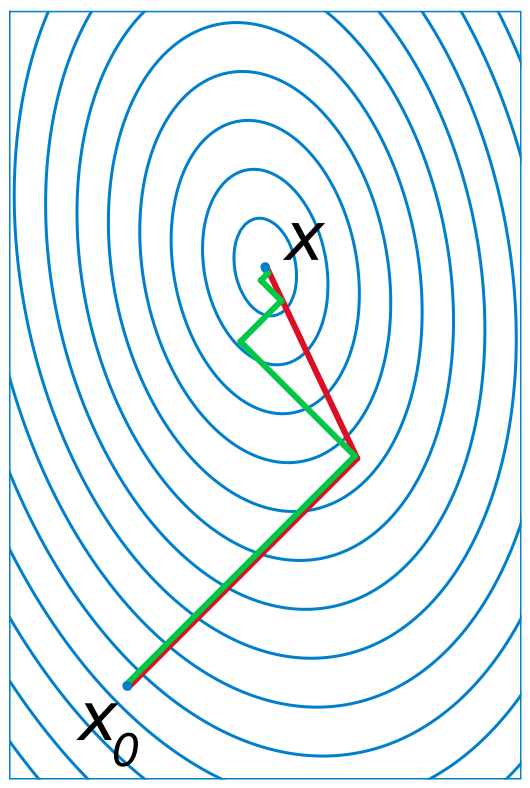
\includegraphics[width=0.3\linewidth]{images/project with Wiem/Conjugate_gradient_illustration.png}
    \caption{Visualization of the advantage of the CG method compared to GD: CG requires significantly fewer steps. The green line shows the path of the GD method, red shows the path of the CG method. Image from Wikipedia.org.}
    \label{fig:CG_vs_GD}
\end{figure}

\subsection{Nonlinear Conjugate Gradient Method}
Our problem, however, is nonlinear, so the CG method described above needs some further adjustment. Therefore, the nonlinear conjugate gradient (NCG) method is used to minimize the cost function $f(\mathbf{x})$, and thus reconstruct the image:
$$\mathbf{x}_{k+1} = \mathbf{x}_k + \alpha_k \mathbf{d}_k$$
\begin{align*}
    \mathbf{d}_k &=
    \begin{cases}
    -\mathbf{g}_k & k = 1 \\
    -\mathbf{g}_k + \beta_k \mathbf{d}_{k-1} & k > 1
    \end{cases},
\end{align*}
where $\mathbf{g}_k$ denotes the gradient at the $k$th step.

While that method appears to be even simpler than the CG method, unfortunately, there is no optimal way to calculate $\alpha_k$ and $\beta_k$ parameters, so multiple methods are proposed. The two main conditions of a good method are the following:
\begin{itemize}
    \item Descent property:
    \begin{itemize}
        \item Strict: Cost function must strictly decrease in each step ($\mathbf{g}_k \mathbf{d}_k < 0$)
        \item Sufficient: We can allow a certain amount of increase in cost function ($\mathbf{g}_k \mathbf{d}_k < -c ||\mathbf{g}_k||^2$)
    \end{itemize}
    \item Global convergence
    \item Fast convergence
\end{itemize}
While it is practically impossible to fully satisfy all these three conditions at the same time, but these can be used to compare the different methods.

1) To get the $\alpha_k$ parameter, the most commonly used method is line search:
$$\alpha_k = \argmin_{\alpha > 0} f(\mathbf{x}_k + \alpha_k \mathbf{d}_k).$$
Since exact line search is usually expensive and impractical, the strong Wolfe line search is often considered in the implementation of nonlinear conjugate gradient methods. It aims to find a step size satisfying the strong Wolfe conditions:
$$f(\mathbf{x}_k + \alpha_k \mathbf{d}_k) - f(\mathbf{x}_k) \leq \rho \alpha_k \mathbf{g}_k \mathbf{d}_k$$
$$|g(\mathbf{x}_k + \alpha_k \mathbf{d}_k)^T \mathbf{d}_k| \leq - \sigma \mathbf{g}_k^T \mathbf{d}_k.$$
One method to find an $\alpha$ satisfying the Wolfe conditions is backtracking line search, where the "query" point is initially moved to a certain distance from the current location along the selected direction, and then that distance is decreased in each step until the local minimum is reached.
Fig.~\ref{fig:backtracking} visualizes that method in case of a simple quadratic function.

\begin{figure}
    \centering
    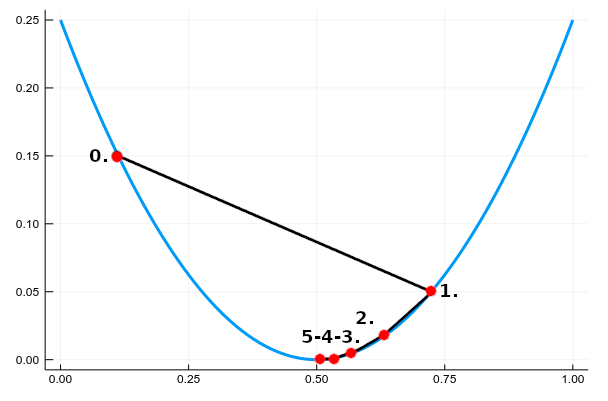
\includegraphics[width=0.3\linewidth]{images/project with Wiem/backtracking.png}
    \caption{Example of backtracking line search.}
    \label{fig:backtracking}
\end{figure}

2) Similarly, to obtain the $\beta_k$, there are multiple choices. The oldest method is the Fletcher-Reeves (FR) method:
$$\beta_k^{FR} = \frac{||\mathbf{g}_k||^2}{||\mathbf{g}_{k-1}||^2}.$$
The advantage of that method that global convergence is proved for $\sigma < \frac{1}{2}$ in the Wolfe condition using inexact line search~\cite{Al-Baali}. However, the convergence is relatively slow in many cases because it may fall into some circle of tiny steps, so that method is significantly outperformed by the Polak-Ribi\`{e}re-Polyak (PRP) method:
$$\beta_k^{FR} = \frac{\mathbf{g}_k^T (\mathbf{g}_k - \mathbf{g}_{k-1}}{||\mathbf{g}_{k-1}||^2}.$$
In spite of the improved speed, that method also has a serious problem: Global convergence can only be proved for strictly quadratic functions. There exist some sophisticated line search method that ensures global convergence for all nonlinear functions, but these methods are also computationally more intensive~\cite{grippo}.
To overcome that problem, one can improve the convergence compared to FR method speed (but reduce compared to PRP) while keeping the global convergence property for Wolfe line search by combining the two methods: $\beta_k^{GN} = \max\{-\beta_k^{FR}, \min\{\beta_k^{PRP},\beta_k^{FR}\}\}.$
Although there are multiple newer methods that are more efficient, these methods fall out of the scope of that study.

3) To sum up, the algorithm used in \cite{sparse} is the following ($TolGrad$, $maxIter$, and $\mu$ variables are parameters to control the precision):
\begin{algorithm}[H]
 // Initialization:\\
 $k \leftarrow 0$; $m \leftarrow 0$; $\mathbf{g}_0 \leftarrow \nabla f(\mathbf{x}_0);  \mathbf{d}_0 \leftarrow - \mathbf{g}_0$\;
 -------------------------------------------------------------------- \\
 // Iterations:\\
 \While{$||\mathbf{g}_k\|_2 < TolGrad$ and $k > maxIter$}{
  // Backtracking line search\\
   ~~~~~~~(inner loop condition: 1st Wolfe condition)\\
  $\alpha_k \leftarrow 1$\\
  \While{$f(\mathbf{x}_k + t  \mathbf{d}_k) - f(\mathbf{x}_k) > \rho \alpha_k \cdot \mathbf{g}_k^*  \mathbf{d}_k$}{
    $\alpha_k \leftarrow \mu \cdot \alpha_k$\\
  }
 ---------------------------------------------------------------- \\
  // Changing position along the selected direction using the calculated $\alpha_k$\\
  $\mathbf{x}_{k+1} \leftarrow \mathbf{x}_{k} + \alpha_k \mathbf{d}_{k}$\\
 ---------------------------------------------------------------- \\
  // Calculate next direction\\
  $\mathbf{g}_{k+1} \leftarrow \nabla f(\mathbf{x}_{k+1})$\\
  $\gamma \leftarrow \frac{||\mathbf{g}_{k+1}||_2^2}{||\mathbf{g}_{k}||_2^2}$ // Fletcher-Reeves method\\
  $ \mathbf{d}_{k+1} \leftarrow - \mathbf{g}_{k+1} + \gamma \mathbf{x}_{k}$\\
  $k \leftarrow k + 1$\\
 }
\end{algorithm}


\subsection{Proximal Methods}
Proximal operator, Iterative Shrinkage/Soft Thresholding Algorithm, Forward-Backward Splitting with linear line search, Wolfe conditions

To solve the optimization problem that leads to image reconstruction, a simple and widely applied method is the gradient descent and its derivatives (e.g. conjugate gradient); however, they cannot be applied simply in our case because the cost function
$$f(\mathbf{x}) = \frac{1}{2} \sum_{\ell = 1}^L \sigma_\ell^{-2} \|F_\Omega \mathbf{S}_\ell \mathbf{x} - \mathbf{y}_\ell \|_2^2 + \lambda \|\mathbf{\Phi x} \|_1$$
does not have a derivative as the $\ell^1$ norm cannot be differentiated.
Finding a both universal and efficient method to solve constrained optimization problems, where either cost function or constraint does not have a gradient, is still unsolved, but we can solve that issue by restricting the class of problems to those that has the following general Lagrangian form:
$$\mathbf{\hat{x}} = \argmin_{x \in \mathcal{H}} \{E(\mathbf{x}) + R(\mathbf{x})\},$$
where $E(\mathbf{x})$ (empirical error) is continuously differentiable convex function with $\beta$-Lipschitz continuous gradient ($\|f(\mathbf{x}) - f(\mathbf{y})\| \leq \beta \|x - y\| : \forall \mathbf{x}, \mathbf{y} \in \mathbb{C}^N$), and $R(\mathbf{x})$ (regularization term) is a non-smooth, continuous function. For that class of problems, we can define the proximity operator instead of the gradient to find a local minimum in the proximity of the current location:
$$prox_f(\mathbf{v}) := \argmin_x \frac{1}{2} \|\mathbf{x} - \mathbf{v} \|_2^2 + f(\mathbf{x}).$$

\subsection{Forward-backward splitting}
One possible implementation of proximity gradient method is forward-backward splitting (FB), which consists of two consecutive steps: First, the "forward step" that optimizes $E(x)$ with gradient ($\mathbf{w}_{k+1} = \mathbf{x}_k - t_k \nabla E(\mathbf{x}_k)$), then the "backward step" optimizes $R(\mathbf{x})$ by proximity operator ($\mathbf{x}_{k+1} = prox_R(\mathbf{w}_{k+1})$). That two steps can be merged into one formula:
$$\mathbf{x}_{k+1} = prox_R(\mathbf{x}_k - t_k \nabla E(\mathbf{x}_k)).$$

\subsection{ISTA: Iterative Shrinkage-Thresholding Algorithm}
The most difficult part of FB splitting is the calculation of proximity operator in general. However, the problem can be tremendously simplified by restricting regularization term to $\ell^1$-norm, also known as LASSO (least absolute shrinkage and selection operator) regularization: $R(\mathbf{x}) = \lambda ||\mathbf{\Phi x} ||_1$. That way the proximity operator can be simplified to soft-thresholding function~\cite{combettes_wajs_2005}:
$$soft(x,c) = sign(x) \cdot max(|x| - c, 0).$$
Fig.~\ref{fig:soft-thres} shows an example for soft-thresholding functions. Because of that name, the algorithm is also commonly referred as iterative \textit{soft}-thresholding algorithm. In that special case of FB splitting, it is even possible to determine an upper bound for convergence, which is $\mathcal{O}(\frac{1}{\epsilon})$ in that case~\cite{FISTA}.

\subsection{Relaxed Forward-Backward}
While ISTA is a well-known and widely used optimization method, its convergence speed can be vastly improved by taking the "momentum" into account. As the name implies, there is an analogy from physics that explains well how that method works: Let's imagine a ball rolling down from a hill. That ball, obviously, always try to follow the gradient, but as it rolls down in one direction, it also gains speed, thus momentum and kinetic energy. If the direction gradient changes frequently, than the ball also changes directions often, and it cannot gain speed. But if there is a straight slope, then the ball gathers kinetic energy, and it takes more time to change the direction even if the direction of the gradient changes.

That phenomenon can be expressed by the momentum term, which is basically the numerical derivative of the position, and we adjust the current position by that term:
$$x_k = prox_{ \gamma || \cdot ||_1}(z_k - \frac{1}{L} \nabla E(z_k)),$$
$$z_{k+1} = x_k + \mu (x_k - x_{k-1}),$$
where $\mu$ is the weight that balances the effect of momentum and gradient. However, determining the $\mu$ value is not trivial, and the optimal value depends on the problem. Such a measurement that searches for the optimal value is presented in~\cite{peyre_2011}, and fig.~\ref{fig:mu} shows the result.

%\begin{figure}
%    \centering
%    \includegraphics[width=0.5\linewidth]{relaxed-FB.png}
%    \caption{Speed of convergence for different $\mu$ values. %Image from~\cite{peyre_2011}.}
 %   \label{fig:mu}
%\end{figure}

\subsection{FISTA: Fast Iterative Shrinkage-Thresh. Algorithm}
Whereas introducing momentum rule leads to significant gain in convergence speed, the upper bound of convergence is still $\mathcal{O}(\frac{1}{\epsilon})$, and determining an optimal $\mu$ is a problem, as well. However, Beck et al.~\cite{FISTA} presented a method that can determine $\mu$ easily in such a way that the rate of convergence is $\mathcal{O}(\frac{1}{\epsilon^2})$, which is the theoretical limit defined by Nesterov~\cite{nesterov_1983} for optimization methods:
$$x_k = prox_{ \gamma || \cdot ||_1}(z_k - \frac{1}{\beta} \nabla E(z_k)),$$
$$\tau_k = \frac{1 + \sqrt{1 + 4(\tau_{k-1})^2}}{2},$$
$$\mu_k = \frac{\tau_{k-1} - 1}{\tau_k},$$
$$z_{k+1} = x_k + \mu_k (x_k - x_{k-1}),$$
where $\beta$ can easily calculated by power iteration method (eigenvalue decomp.) because of NFFT.

The reason why that method is significantly faster than the previous method is that $\mu$ value changes through the optimization, so the effect of momentum is small in the beginning of the optimization process (as the gradient is large enough to provide good convergence speed), but later the importance of momentum is gradually increasing because the surface of cost function is flat around the solution in most cases (see fig.~\ref{fig:mu_FISTA}). That method provides even faster convergence than relaxed FB, and also solve the problem of finding optimal $\mu$ value. Fig.~\ref{fig:ISTA_vs_FISTA} shows a comparison of converge speed in case of a simple optimization problem presented in~\cite{peyre_2011}.

%\begin{figure}
 %   \centering
 %   \includegraphics[width=0.5\linewidth]{mu.png}
 %   \caption{Change of $\mu$ value during optimization steps.}
 %   \label{fig:mu_FISTA}
%\end{figure}

%\begin{figure}
 %   \centering
 %   \includegraphics[width=0.5\linewidth]{ISTA_vs_FISTA.png}
 %   \caption{Comparism of convergence speed of FB, relaxed FB, %and FISTA methods. Image from~\cite{peyre_2011}.}
 %   \label{fig:ISTA_vs_FISTA}
%\end{figure}

\subsection{FOGM: Proximal Optimized Gradient Method}
Another method to increase convergence speed is proposed in~\cite{hendrickx_2018}, which was further improved in~\cite{gueddari_2018}. The main features of that method is that it gives a changing weight ($\gamma_k$) to the proximity operator, uses a more advanced form momentum rule, and it increases $\tau$ value in the last two steps increasing the effect of momentum at the same time that helps to avoid the slowdown of the convergence in the flat area around the solution. Although these modifications do not change the theoretical lower bound for convergence speed ($\mathcal{O}(\frac{1}{\epsilon^2})$), they make the algorithm having an about two-times faster worst-case convergence speed compared to FISTA~\cite{kim, taylor}. The steps of that algorithm are the following:

\begin{algorithm}[H]
 $k \leftarrow 0$; $\tau_0 \leftarrow 1$; $\mathbf{y}_0, \mathbf{z}_0 \leftarrow$ arbitrary value\;
 \While{$k \leq K - 1$}{
  \eIf{$k < K - 1$}{
    $\tau_k \leftarrow \frac{1 + \sqrt{1 + 4(\tau_{k-1})^2}}{2}$\\
  } {
    $\tau_k \leftarrow \frac{1 + \sqrt{1 + 8(\tau_{k-1})^2}}{2}$ // Extra speed in last two steps\\
  }
  $\gamma_{k+1} \leftarrow \frac{1}{\beta} \frac{2\tau_k + \tau_{k+1}-1}{\tau_{k+1}}$ // Weight for the proximity operator\\
  $\mathbf{x}_{k+1} \leftarrow \mathbf{z}_k - \frac{1}{\beta} \nabla E(\mathbf{z}_k)$ // Move along the gradient\\
  $\mathbf{z}_{k+1} \leftarrow \mathbf{x}_{k+1} + \frac{\tau_{k} - 1}{\tau_{k+1}} (\mathbf{x}_{k+1} - x_k) + \frac{\tau_k}{\tau_{k+1}}(\mathbf{x}_{k+1} - \mathbf{y}_k) + \frac{\tau_k - 1}{\beta \gamma_k \tau_{k+1}}(\mathbf{z}_k - \mathbf{y}_k)$ // More advanced momentum rule\\
  $\mathbf{y}_{k+1} \leftarrow prox_{\gamma_{k+1}}(\mathbf{z}_{k+1})$\\
  $k \leftarrow k + 1$\\
 }
\end{algorithm}

\subsection{ADMM}
what is it and why is it good

\fi